\section{Sliding Game}
Our metric for algorithmic performance involves running A* on the sliding game (see the Youtube video for a demonstration). The sliding game is a particularly convenient search problem for two reasons: the state representation is small and the state space is very large. It blows up exponentially with respect to the puzzle dimensions. This is particularly important since our goal was to measure the effectiveness of a parallel A* algorithm, and the expansive state space would decrease potential overhead.
\newline\newline
\begin{tabular}{ |p{3cm}||p{3cm}|p{3cm}|p{3cm}|  }
\hline
\multicolumn{4}{|c|}{Sliding Game Sequential Execution times} \\
\hline
Board Size& Runtime (ns)&Runtime (ms)& Runtime (s)\\
\hline
2x3 & 35880 & 0 & 0\\
3x3 & 84711 & 0 & 0\\
3x4 & 258638033 & 259 & 0\\
4x4 & 171623957677 & 171624 & 172\\
\hline
\end{tabular}
\newline
\begin{figure}[h]
    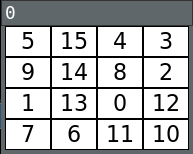
\includegraphics[scale=0.5]{figures/4x4.png}
    \caption{The puzzle grid used for the 4x4 measure}
    \label{fig:gastar_ds}
\end{figure}
\newline
The object of the game is to order the tiles in increasing numerical order. The 0 tile represents an empty tile where adjacent tiles can "slide" to. Thus, every turn can result in 4 more possible states (exponential). The graph below is a visual representation of the above runtimes in log scale.

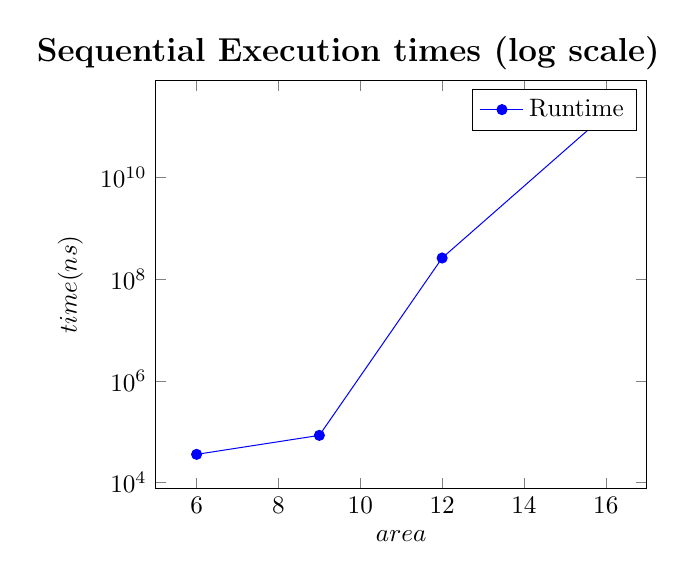
\begin{tikzpicture}[scale=0.91]
    \begin{axis}[
        xlabel=$area$,
        ylabel=$time(ns)$,
        ymode=log
                ]
    \addplot[mark=*,blue] plot coordinates {
        (6,35880)
        (9,84711)
        (12,258638033)
        (16,171623957677)
    };
    \addlegendentry{Runtime}
   
    \end{axis}
    \node[above,font=\large\bfseries] at (current bounding box.north) {Sequential Execution times (log scale)};
\end{tikzpicture}

\section{Evaluating Performance}
For this problem, we evaluated our implementations by checking the wall time of the implementations. We found this to be appropriate for the serial algorithm given that we were not able to properly evaluate speedup for the GA* GPU method.

\section{Scaling the Problem Space}
Considering our sequential performance in the graph above, we see that the line is roughly linear. This supports our hypothesis that as the number of cells grow, the runtime grows roughly exponentially. In particular, we see that because most nodes on the frontier have 3 or 4 neighbors, the number of states being added as we go further from the initial state increases exponentially. Due to the nature of the problem, a small change in workload could result in dramatically larger runtime.

\section{Limitations of our Approach}
The main source of issues with our CUDA implementation came from our hash map. Our implementation of the hash map involves a table and two hash functions where the second can search for new locations in the table for a node if another element collides with it per the first hash function. Although this simplification allows us to not need sychronization in this section, it means that we need a very large hash table. If the hash table is small compared to the number of states, it is possible that an element has collisions with both the hash functions. In this case, the hash map will \textit{lose information} that could potentially be important for the final path.\newline\newline
Another limitation of our approach was the amount of global memory that we allocate in this method. We use it for the large array \verb|S| as well as the hash table. If we scale up the hash table size in order to reduce the likelihood of collisions, we will increase the global memory allocated. In the GPU, global memory is far less efficient to update than shared memory. \textbf{As a result, the global memory brought upon by the hash table would likely be our main bottleneck in the CUDA implementation.}

\section{Changing the Hardware}
As we have discovered through this project, a GPU implementation of A* is not too pragmatic. In particular, the memory constraint of GPUs especially for search problems of this magnitude is quite restrictive. In contrast, using MPI would alleviate this. \textbf{MPI is not restricted by a single device and can be used across a network of devices, thus relaxing the space constraints}. Furthermore, MPI is a more task oriented system whereas CUDA is more data oriented, which is more suitable for search problems.